\input ../SlidePreamble
\input ../preamble


\begin{document}

{\Huge
  \centerline{\bf TTIC 31230,  Fundamentals of Deep Learning}
  \vfill
  \centerline{David McAllester, Winter 2020}
  \vfill
  \centerline{\bf Pretraining for NLP}
  \vfill
  \vfill

\slide{Pretraining for NLP}

In NLP unsupervised pretraining is now required for strong benchmark performance.


\slide{Pretrained Word Embeddings}

Advances in Pre-Training Distributed Word Representations, Mikolov et al., 2017

\vfill
We want a mapping from a word $w$ to a vector $e(w)$ --- a word embedding.

\vfill
{\color{red} fastText} from Facebook is currently popular.

\vfill
It provides both contextual bag of words (cbow) and byte pair encoding (BPE) word vectors.

\slide{cbow word vectors}

We construct a population distribution on pairs $(c,w)$ here $c$ is a bag of word context and $w$ is a word.

\vfill
$$\Phi^* = \argmin_\Phi E_{c,w}\;-\ln P(w|c)$$

\vfill
$\Phi$ consists of a matrix $e[w,i]$ where $e[w,I]$ is the word embedding of $w$, and a matrix $e'[w,i]$ giving the embedding of the word
$w$ when it appears in a context.

\vfill
A score $s(w|c)$ is defined by
$$s(w|c) = \frac{1}{|c|} \sum_{w' \in c}\;e(w)^\top e'(w')$$

\slide{Negative Sampling in cbow}

\vfill
Rather than define $P_\Phi(w|c)$ by a softmax over $w$, one uses restricted negative sampling.

\vfill
We construct a training set of triples $(w,c,N_C)$

\vfill
$$\Phi^* = \argmin_\Phi\;E_{w,c,N_c}\;\ln\left(1 + e^{-s(w,c)}\right) + \sum_{n \in N_C} \ln\;\left(1 + e^{s(n,c)}\right)$$

\slide{Byte Pair Encoding (BPE)}

BPE constructs a set of character n-grams by starting with the unigrams and then greedily merging most common bigrams of n-grams.

\vfill
Given a set of character n-grams each word is treated as a bag of character n-grams.

\vfill
$$e[w] = \frac{1}{N} \sum_{n \in w}\; e(n)$$

\vfill
Current systems use byte pairs but train the byte pair embeddings as part of transformer training.


\slide{BERT: Blank Languagage Modeling}

We replace a random subset of the words with a blank token.

\vfill
We run a transformer on a block of text containing some blanks.

\vfill
For a blank occurring at position $t$ we predict the word at position $t$:

\vfill
$$P(w) = \softmax_w\;h[t,J]e[w,J]$$

\vfill
Blank language modeling outperforms language modeling when used for pretraining in classification tasks such as the GLUE tasks.


\slide{GLUE}

GLUE: General Language Understanding Evaluation

\vfill

\centerline{\normalsize ArXiv 1804.07461}
\centerline{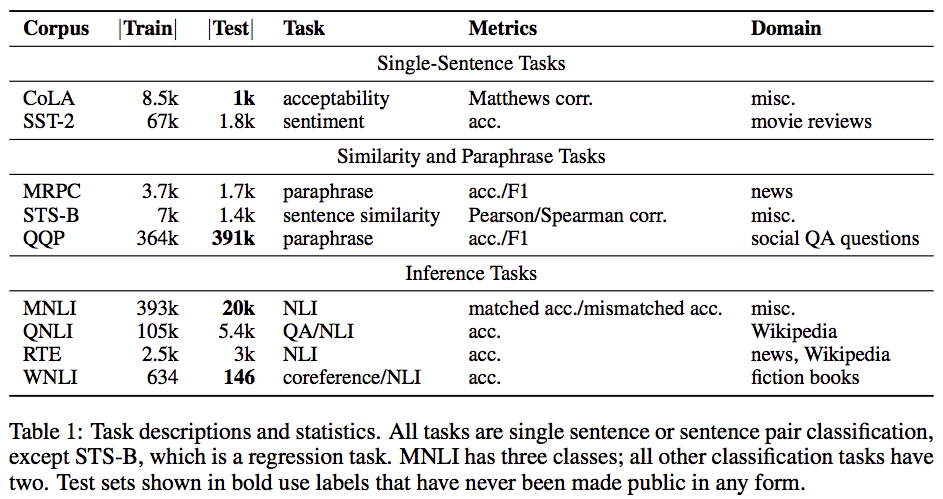
\includegraphics[width= 7in]{\images/GLUE}}

\slide{GLUE Leader Board as of February 27, 2020}

\centerline{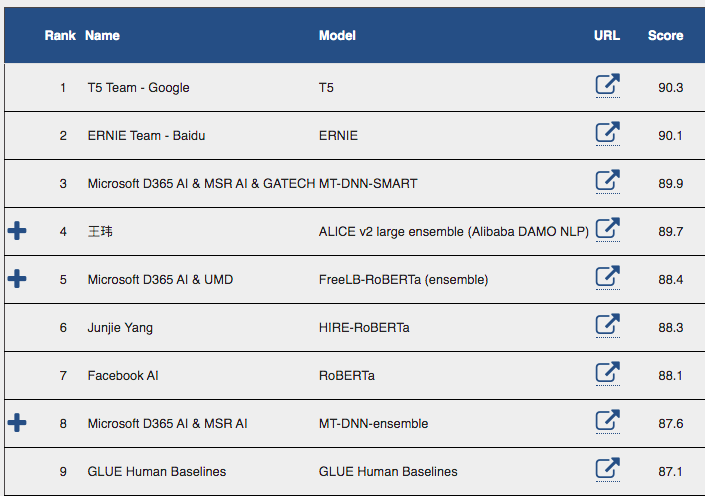
\includegraphics[width= 7in]{\images/GLUELeader}}

\slide{SuperGLUE Leader Board as of February 27, 2020}

\centerline{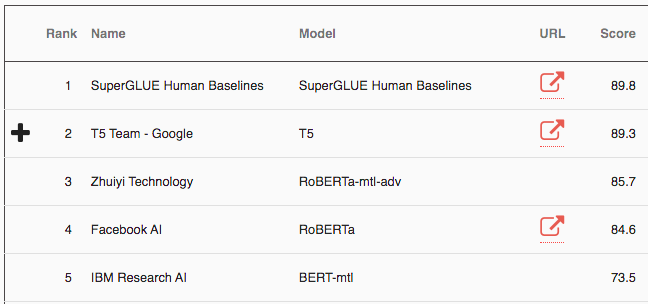
\includegraphics[width= 9in]{\images/SuperLeader}}

\slide{Fine Tuning on Question Answering}

COMET: Busselut et al, June 2019.

\vfill
Charlie is drifting though life:

\centerline{\includegraphics[height=4in]{\images/COMET}}\

\slide{The Chatbot Meena}

\centerline{\includegraphics[height=4in]{\images/meena1}}\

\slide{The Chatbot Meena}

\centerline{\includegraphics[height=4in]{\images/meena2}}\


\slide{END}

}
\end{document}
